\subsection{Abstract Factory (\textit{o Kit})}
\label{abstract-factory}

\textbf{Scopo}: Creazionale \\
\textbf{Raggio d'azione}: Oggetti

\paragraph{Definizione} \textbf{Object Creational} Fornisce un’interfaccia per la creazione di famiglie di oggetti correlati o dipendenti senza specificare quali siano le loro classi concrete.

\paragraph{Motivazione} Si consideri lo sviluppo di un toolkit per la realizzazione di GUI in grado di supportare diversi look-and-feel. Affinché sia possibile il codice che la implementa non deve dipendere dal tipo specifico dei widget utilizzati quindi non può istanziarli direttamente.

\begin{figure}[H]
    \centering
    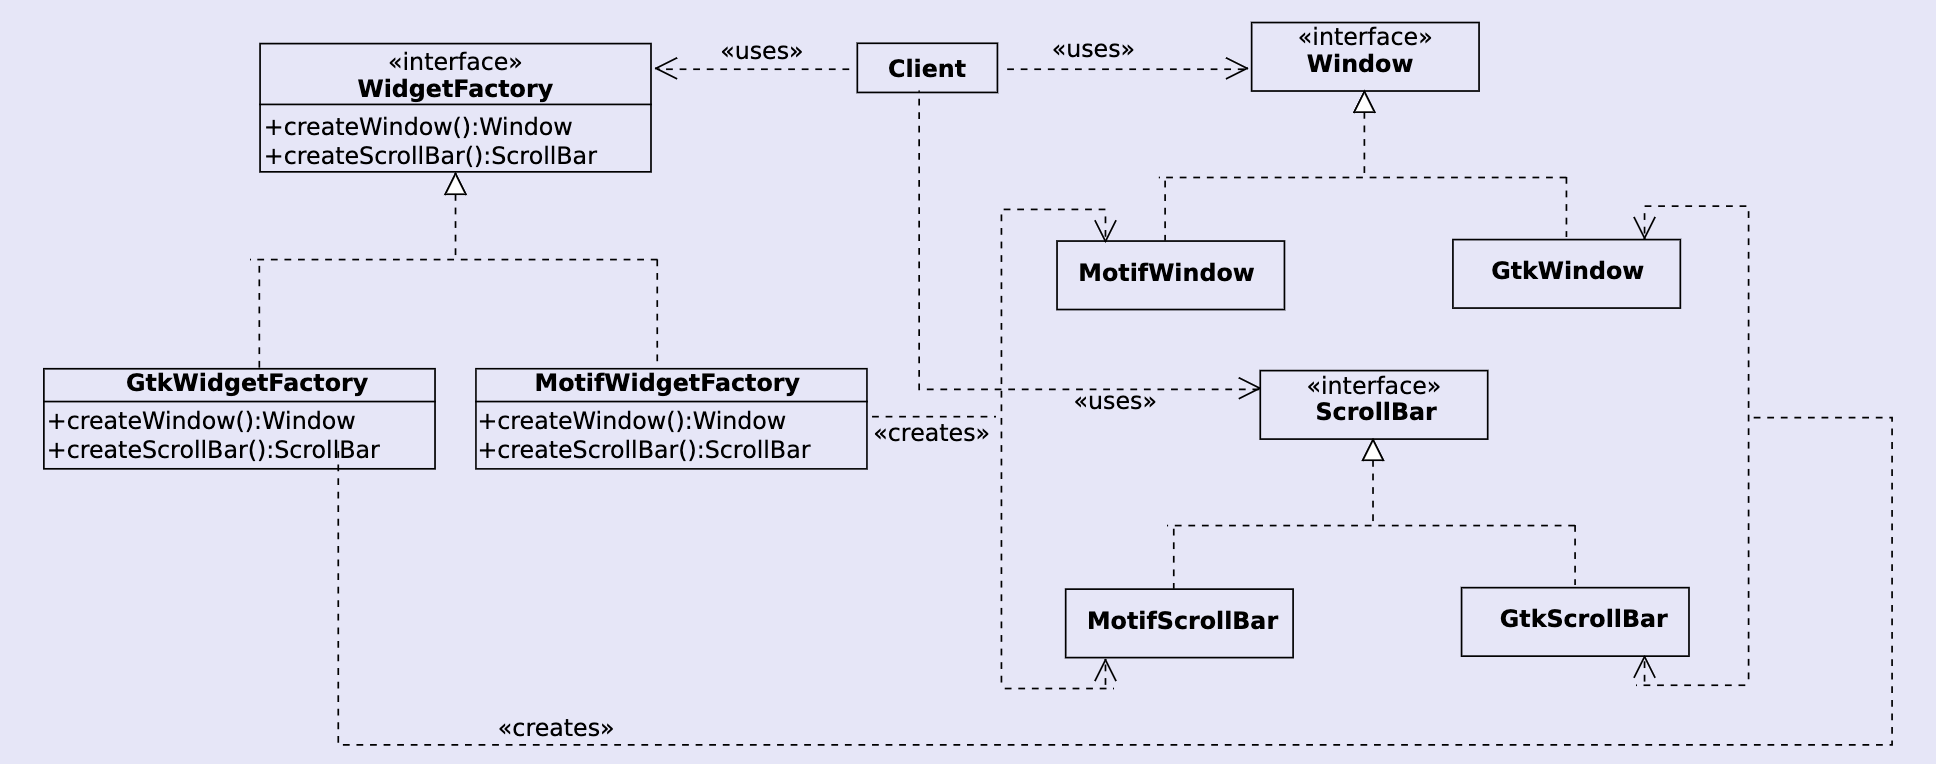
\includegraphics[width=0.75\linewidth]{assets/pattern/abstract-factory/abstract-factory-esempio.png}
\end{figure}

L’interfaccia WidgetFactory introduce un metodo per la creazione di ciascun tipo di base di widget definito a sua volta da un’oportuna interfaccia. I client invocano i metodi definiti da WidgetFactory per ottenere istanze di widget senza conoscere la classe concreta che utilizzano. Esiste una classe concreta che implementa WidgetFactory per ciascuno dei L\&F considerati.

\begin{figure}[H]
    \centering
    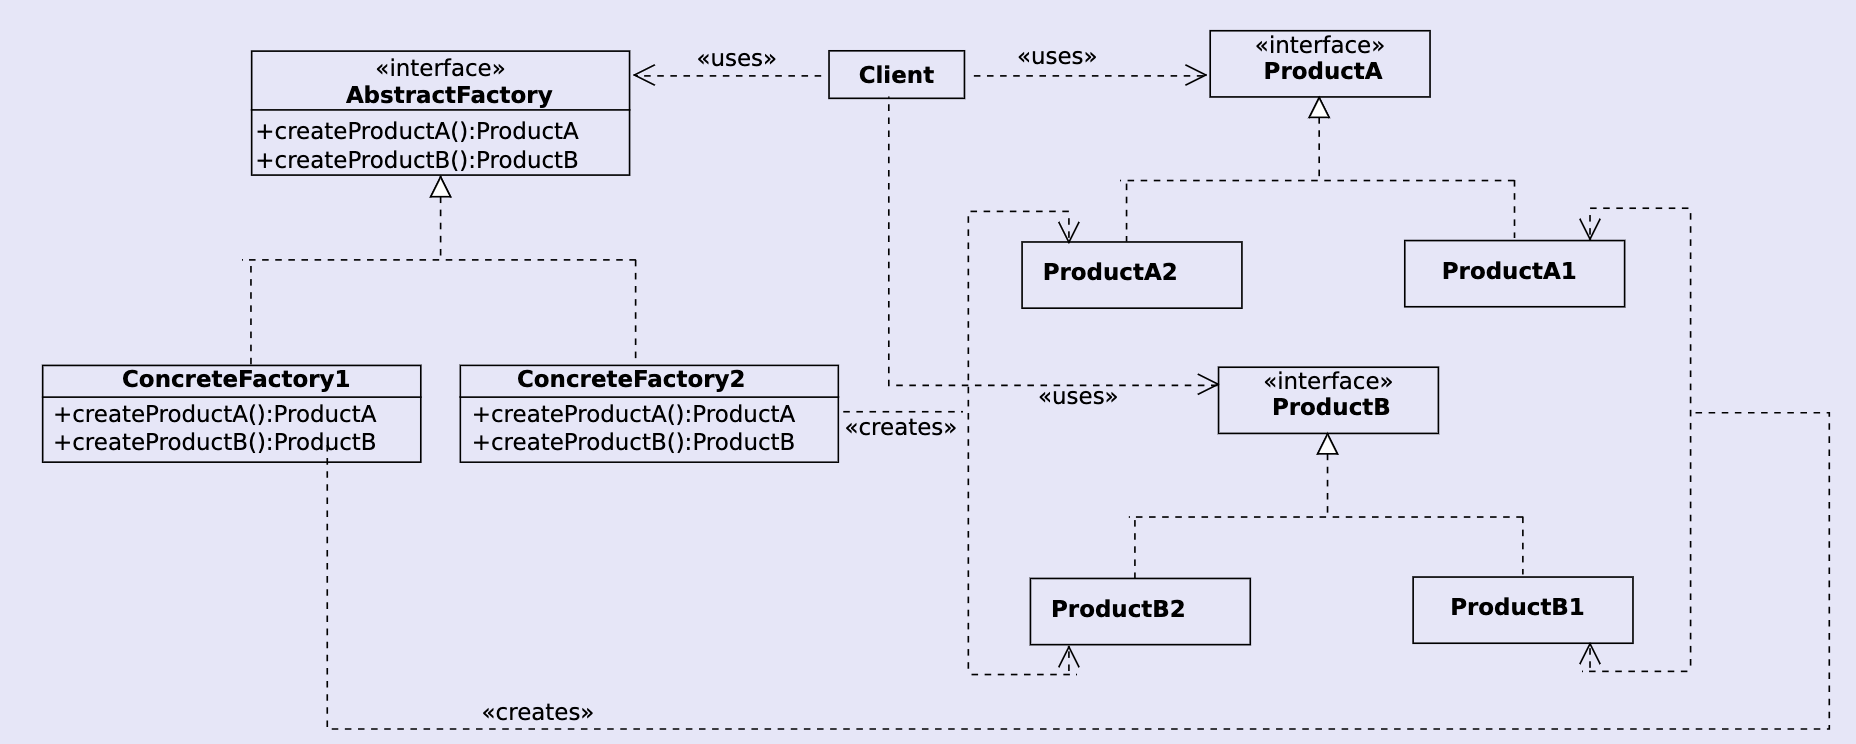
\includegraphics[width=0.75\linewidth]{assets/pattern/abstract-factory/abstract-factory-struttura.png}
    \caption{Class Diagram del pattern Abstract Factory}
\end{figure}

\paragraph{Applicabilità} È consigliabile utilizzare il pattern AbstractFactory quando:
\begin{itemize}
    \item Un sistema deve essere indipendente dai processi di creazione, composizione e rappresentazione di un oggetto o famiglia di oggetti;
    \item Un sistema deve essere configurato con una o più famiglie di prodotti (oggetti);
    \item Una famiglia di oggetti è stata disegnata con l'intento di farli funzionare insieme;
    \item Si vuole fornire una libreria di prodotti dei quali si vuole rendere nota la sola interfaccia.
\end{itemize}

\paragraph{Struttura} I partecipanti del pattern sono:
\begin{itemize}
    \item \textbf{AbstractFactory} (WidgetFactory): dichiara un’interfaccia per le operazioni di creazione di oggetti (possibilmente implementate tramite FactoryMethod \ref{factory-method}) prodotto astratti.
    \item \textbf{ConcreteFactory} (MotifWidgetFactory, GtkWidgetFactory): implementa le operazioni degli oggetti prodotto concreti.
    \item \textbf{AbstractProduct} (Window, ScrollBar): dichiara un’interfaccia per un tipo di prodotti
    \item \textbf{ConcreteProduct} (MotifWindow, GtkWindow): implementa l’interfaccia Product definendo un oggetto prodotto creato dalla corrispondente factory concreta.
\end{itemize}

Per creare oggetti (prodotti) diversi, i client dovrebbero usere ConcreteFactory diverse.
AbstractFactory delega la creazione alle sue ConcreteFactory.

\paragraph{Conseguenze} Il pattern AbstractFactory consente quindi di:
\begin{itemize}
    \item \textbf{Isolare le classi concrete}: processo di creazione incapsulato nella Factory.
    \item \textbf{Cambiare agilmente la famiglia di prodotti utilizzata}: cambio di configurazione cambiando il tipo di Factory, della quale è prevista una sola istanza (Singleton \ref{singleton}).
    \item \textbf{Promuovere la consistenza nell'utilizzo dei prodotti}: l'applicazione utilizza una sola famiglia di prodotti per volta.
    \item \textbf{Rende complicato implementare nuove famiglie di prodotti}: prevede il cambiamento dell'AbstractFactory e di conseguenza anche tutte le ConcreteFactory che la implementano.
\end{itemize}

\begin{figure}[H]
    \centering
    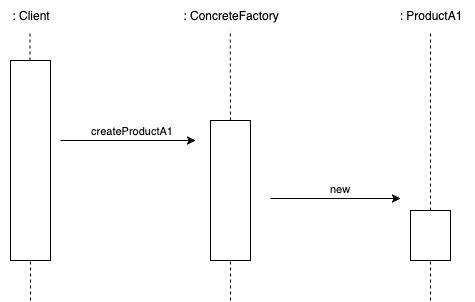
\includegraphics[width=0.75\linewidth]{assets/pattern/abstract-factory/abstract-factory-sequence.drawio.png}
    \caption{Sequence Diagram del pattern Abstract Factory}
\end{figure}

\newpage